\chapter{第4章 P公司小微贷款服务质量评价模型构建与测量}

本章承担DMAIC方法论中"测量"（Measure）阶段的核心任务：在前三章完成问题界定和服务现状诊断的基础上，构建适用于小微信贷服务场景的质量评价模型，通过问卷调查获取客户期望与感知的双向数据，以量化方式定位P公司小微贷款服务质量的核心短板，为第5章的根因分析和改进方案设计提供定量依据。\par

\section{评价模型选择依据}

服务质量评价领域存在多种成熟的测量工具，不同模型的服务场景适配性和诊断能力各有侧重。在正式构建评价体系之前，有必要对主流模型进行系统比较，以确定最适合P公司小微贷款服务质量评价的方法论基础。\par

客户满意度指数（Customer Satisfaction Index，CSI）是应用最广泛的宏观满意度测量工具，通过结构方程模型将客户期望、感知质量、感知价值和客户抱怨等潜变量纳入统一框架。然而，CSI侧重于"总体满意度"这一汇总性结果变量，无法揭示服务过程中各触点的具体差距，对服务短板的诊断能力有限。净推荐值（Net Promoter Score，NPS）以"您向他人推荐本服务的可能性"为单一核心问题，简单直观、便于跨组织对标，但同样只能反映客户忠诚度的整体倾向，无法提供可操作的服务改进指向。\par

相较而言，Parasuraman、Zeithaml和Berry于1988年提出的SERVQUAL模型以"期望-感知差距"为理论内核，将服务质量分解为有形性、可靠性、响应性、保证性和移情性五个维度，通过分别测量客户在接受服务前的期望值（Expectation）和接受服务后的实际感知值（Perception），以差距值（Gap = P - E）作为服务质量的操作化指标\cite{ref21}。该模型的核心理念是：服务质量的高低取决于客户感知与服务期望之间的落差大小，而非单一维度的满意度评分。因此，SERVQUAL天然适合用于诊断服务的具体短板，其诊断逻辑——"哪一维度差距最大，哪一维度就是优先改进对象"——与本文DMAIC方法论中"测量驱动分析、分析驱动改进"的闭环逻辑高度契合。Nguyen等的实证研究进一步表明，服务质量通过客户满意度的中介效应显著影响客户忠诚度，这为以服务质量作为P公司小微贷款业务增长抓手的理论链路提供了支撑\cite{ref26}。\par

在选择SERVQUAL作为基础模型的同时，需要明确其与后续分析工具的组合关系。首先，SERVQUAL提供的是"差距在哪"的诊断信息，而IPA四象限矩阵在此基础上补充了"优先解决什么"的决策框架——将各维度的差距值与客户赋予的重要度权重进行交叉定位，区分出"差距大且重要度高"的优先改进项和"差距大但重要度低"的延迟处理项，从而避免资源投入的均匀分布。其次，AHP层次分析法通过专家两两比较将主观经验判断转化为可供比较的定量权重，解决了IPA中重要度仅依赖客户主观期望这一单一来源的局限性，使优先级的排序更具多视角的稳健性。这一"SERVQUAL测量差距 → IPA交叉定位 → AHP组合赋权"的三层分析链路，构成了本文从测量到识别的完整方法论框架，也与MEM论文强调的工程化管理思维——以定量数据驱动资源分配和决策优化——一以贯之。\par

在银行业和金融服务场景中，SERVQUAL模型已得到广泛应用和验证。花青青等基于SERVQUAL-IPA组合方法对金融机构服务质量进行了系统评价，证实了该模型在金融场景中的信度和效度\cite{ref6}。综合比较三类候选模型的诊断能力、场景适配性和与DMAIC方法论的衔接性，本文选择SERVQUAL作为P公司小微贷款服务质量评价的基础模型，并根据小微信贷服务的特殊性进行必要的维度改良。\par

\section{小微贷款服务质量指标体系构建}

\subsection{维度改良的逻辑}

经典SERVQUAL五维模型（有形性、可靠性、响应性、保证性、移情性）诞生于传统面对面服务场景，而P公司的小微贷款业务具有三个显著差异：其一，服务链路长且环节多，从申请到贷后管理涉及线上平台操作、线下客户经理沟通、后台风控审批等多个界面；其二，信息不对称程度高，客户对费用结构、审批规则、退件原因等敏感信息的透明性有强烈需求；其三，小微客户的异质性大，标准化的贷款产品难以匹配不同生命周期、不同行业客户的差异化资金需求。\par

基于上述场景特殊性，本文在经典SERVQUAL五维基础上新增三个维度：便利性（Convenience），衡量客户在申请、签约、查询等环节的全流程线上化体验和渠道可触达性；透明性（Transparency），衡量客户对费用结构、审批进度和退件原因的知情程度；产品适配（Product Fit），衡量贷款方案与客户经营特征的匹配程度。新增维度参照了Raza等关于线上服务质量维度扩展的研究\cite{ref29}、Zouari等关于数字银行满意度的维度探讨\cite{ref24}以及Kaur等关于数字银行体验与风险的实证分析\cite{ref25}，同时融合了田越\cite{ref11}和孙彦佩\cite{ref12}在国内银行服务质量评价中的指标设计经验，以及P公司内部客户访谈反馈和监管合规要求。\par

最终形成的改良SERVQUAL评价指标体系包含8个维度、32个测量指标，模型框架如图4-2所示。\par

\begin{figure}[htbp]
  \centering
  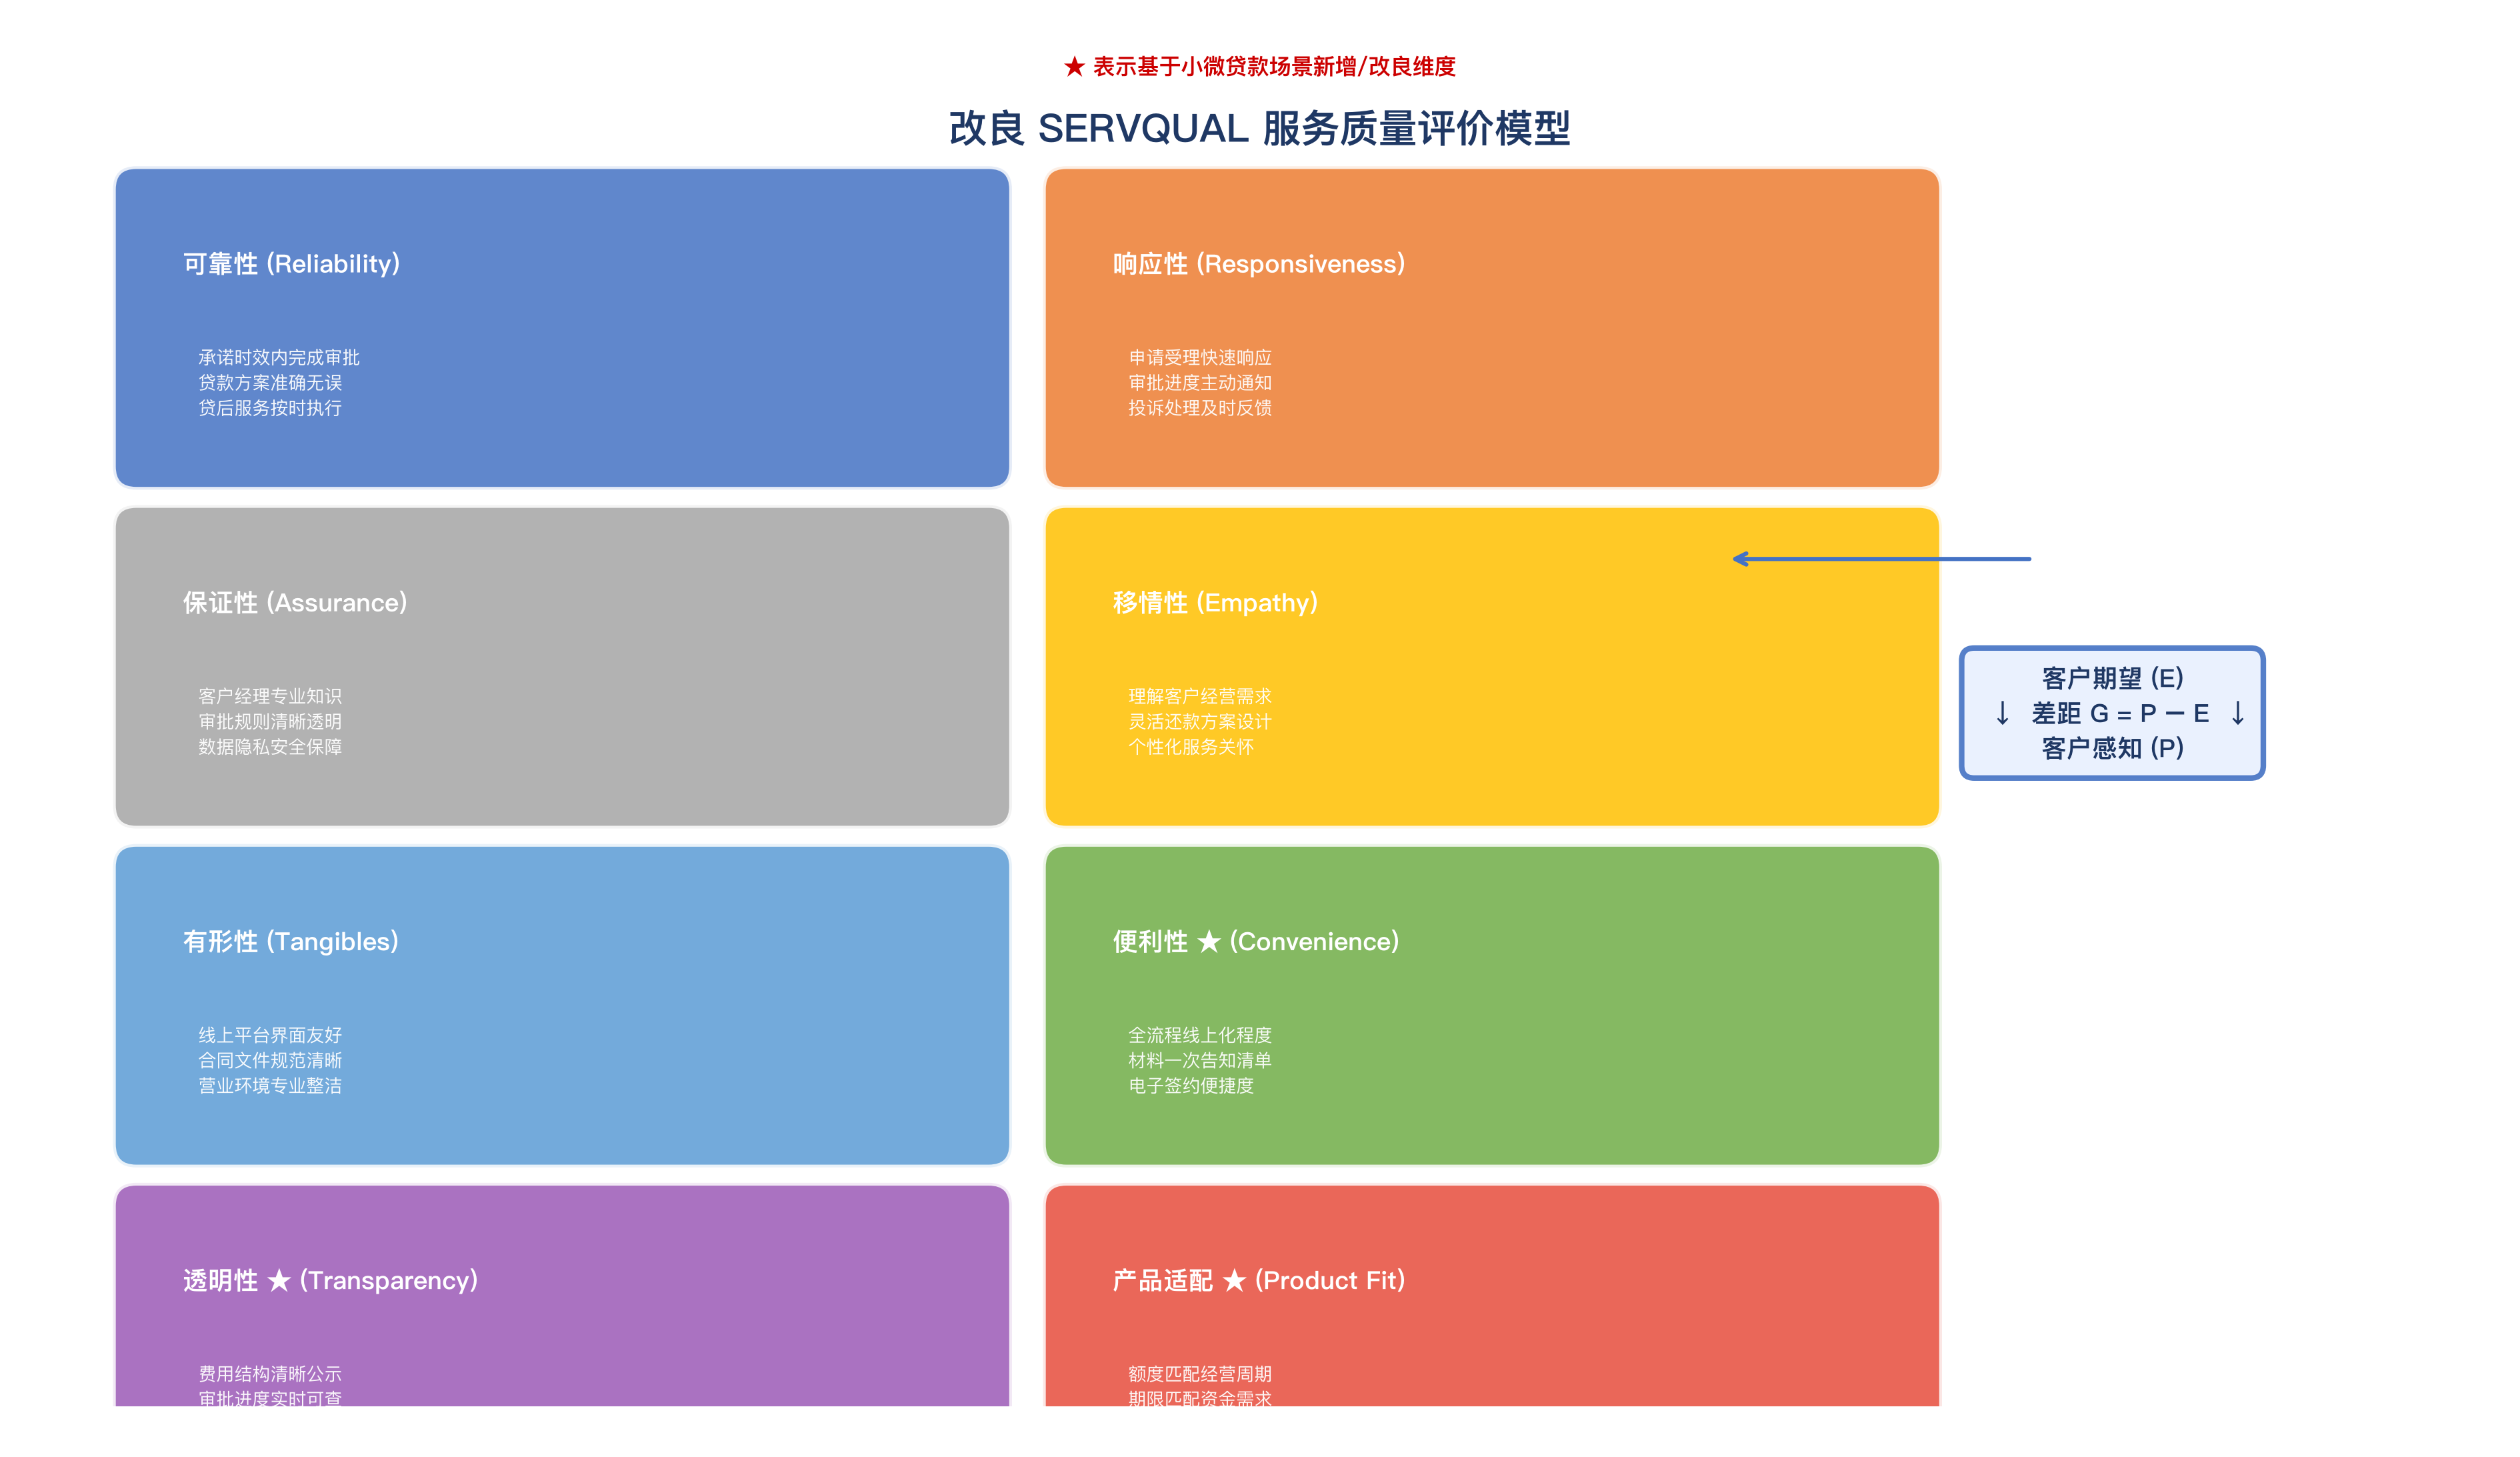
\includegraphics[width=0.85\textwidth]{figures/图4-2_SERVQUAL改良评价指标模型.png}
  \caption{改良SERVQUAL服务质量评价指标模型}
  \label{fig:4-2}
\end{figure}

\subsection{八维32项指标体系}

以下按维度逐一列示指标编号、测量内容和量表来源。各指标均采用李克特五级量表（1=非常不满意/非常不期望，5=非常满意/非常期望），客户分别报告期望值和感知值。\par

（一）可靠性维度（4项）

可靠性衡量服务提供者准确、可靠地履行服务承诺的能力，是小微信贷服务的基础性维度。\par

\begin{table}[htbp]
  \centering
  \small
  \caption{可靠性维度指标体系}
  \begin{tabularx}{\textwidth}{l l l}
    \toprule
    \textbf{编号} & \textbf{指标} & \textbf{量表来源} \\
    \midrule
    SQ01 & 承诺时效内完成贷款审批 & SERVQUAL经典 + 小微场景 \\
    SQ02 & 贷款方案准确无误（额度、利率、期限等） & SERVQUAL经典 \\
    SQ03 & 贷后服务（回访、提醒、结清等）按时执行 & SERVQUAL经典 + 客户反馈 \\
    SQ04 & 投诉处理有明确结论和解决方案 & 客户反馈 \\
    \bottomrule
  \end{tabularx}
\end{table}

（二）响应性维度（4项）

响应性衡量服务提供者主动、及时响应客户需求的能力，直接影响客户的时间成本和焦虑程度。\par

\begin{table}[htbp]
  \centering
  \small
  \caption{响应性维度指标体系}
  \begin{tabularx}{\textwidth}{l l l}
    \toprule
    \textbf{编号} & \textbf{指标} & \textbf{量表来源} \\
    \midrule
    SQ05 & 贷款申请受理后24小时内给予首次响应 & SERVQUAL经典 \\
    SQ06 & 审批进度发生变化时主动通知客户 & 客户反馈 \\
    SQ07 & 拨打客户经理电话3次内能够接通 & 客户反馈 \\
    SQ08 & 投诉受理后24小时内联系客户确认情况 & 客户反馈 \\
    \bottomrule
  \end{tabularx}
\end{table}

（三）保证性维度（4项）

保证性衡量服务人员的专业知识、服务态度及客户对服务安全性的信任程度。\par

\begin{table}[htbp]
  \centering
  \small
  \caption{保证性维度指标体系}
  \begin{tabularx}{\textwidth}{l l l}
    \toprule
    \textbf{编号} & \textbf{指标} & \textbf{量表来源} \\
    \midrule
    SQ09 & 客户经理具备充分的贷款产品知识和风控常识 & SERVQUAL经典 \\
    SQ10 & 贷款审批标准和规则清晰且可理解 & SERVQUAL经典 + 客户反馈 \\
    SQ11 & 客户个人和经营数据的安全有充分保障 & 新增（监管要求） \\
    SQ12 & 客户经理服务态度专业、耐心且友善 & SERVQUAL经典 \\
    \bottomrule
  \end{tabularx}
\end{table}

（四）移情性维度（4项）

移情性衡量服务提供者对客户个性化需求的理解和关怀程度。\par

\begin{table}[htbp]
  \centering
  \small
  \caption{移情性维度指标体系}
  \begin{tabularx}{\textwidth}{l l l}
    \toprule
    \textbf{编号} & \textbf{指标} & \textbf{量表来源} \\
    \midrule
    SQ13 & 客户经理了解客户的经营情况和真实资金需求 & SERVQUAL经典 + 小微场景 \\
    SQ14 & 还款方案（还款日、还款方式等）可根据客户经营周期灵活协商 & 客户反馈 \\
    SQ15 & 贷后主动关心客户的经营状况变化 & SERVQUAL经典 \\
    SQ16 & 在特殊时期（如疫情、自然灾害等）主动提供帮扶方案 & 小微场景新增 \\
    \bottomrule
  \end{tabularx}
\end{table}

（五）便利性维度（★新增，4项）

便利性衡量客户在贷款全流程中的操作便捷度和渠道可触达性，是数字金融服务质量的关键维度。\par

\begin{table}[htbp]
  \centering
  \small
  \caption{便利性维度指标体系}
  \begin{tabularx}{\textwidth}{l l l}
    \toprule
    \textbf{编号} & \textbf{指标} & \textbf{量表来源} \\
    \midrule
    SQ17 & 贷款申请到放款全流程可通过线上完成 & 新增（数字金融趋势） \\
    SQ18 & 申请材料一次性告知且清单明确，无需反复补充 & 客户反馈 \\
    SQ19 & 电子签约流程方便快捷，无需线下往返 & 新增 \\
    SQ20 & 客服可通过多种渠道（App、微信、电话）触达 & 新增 \\
    \bottomrule
  \end{tabularx}
\end{table}

（六）透明性维度（★新增，4项）

透明性衡量客户对贷款服务核心信息的知情程度，是小微信贷服务中信息不对称治理的关键体现。\par

\begin{table}[htbp]
  \centering
  \small
  \caption{透明性维度指标体系}
  \begin{tabularx}{\textwidth}{l l l}
    \toprule
    \textbf{编号} & \textbf{指标} & \textbf{量表来源} \\
    \midrule
    SQ21 & 贷款利率、服务费等费用结构在申请前已清晰说明 & 新增（监管要求） \\
    SQ22 & 贷款审批进度可在线上实时查询 & 客户反馈 \\
    SQ23 & 贷款申请被退回时，退件原因具体、明确 & 客户反馈 \\
    SQ24 & 贷款合同条款表述清晰、易于理解 & 新增 \\
    \bottomrule
  \end{tabularx}
\end{table}

（七）产品适配维度（★新增，4项）

产品适配衡量贷款方案与小微客户经营特征的匹配程度，是提升续贷率和客户黏性的核心维度。\par

\begin{table}[htbp]
  \centering
  \small
  \caption{产品适配维度指标体系}
  \begin{tabularx}{\textwidth}{l l l}
    \toprule
    \textbf{编号} & \textbf{指标} & \textbf{量表来源} \\
    \midrule
    SQ25 & 贷款额度与客户经营规模和资金需求相匹配 & 新增（小微场景） \\
    SQ26 & 贷款期限与客户资金周转周期相匹配 & 新增 \\
    SQ27 & 还款方式灵活可选（等额本息、先息后本等） & 新增 \\
    SQ28 & 贷款到期后的续贷流程便捷高效 & 新增 \\
    \bottomrule
  \end{tabularx}
\end{table}

（八）有形性维度（4项）

有形性衡量服务环境、设备和文件等物理/虚拟载体的专业程度。\par

\begin{table}[htbp]
  \centering
  \small
  \caption{有形性维度指标体系}
  \begin{tabularx}{\textwidth}{l l l}
    \toprule
    \textbf{编号} & \textbf{指标} & \textbf{量表来源} \\
    \midrule
    SQ29 & 线上平台（App/小程序）界面友好、操作流畅 & SERVQUAL经典 + 数字场景 \\
    SQ30 & 贷款合同和申请文件格式规范、清晰 & SERVQUAL经典 \\
    SQ31 & 客户经理着装专业、形象得体 & SERVQUAL经典 \\
    SQ32 & 营业场所环境整洁、设施完善 & SERVQUAL经典 \\
    \bottomrule
  \end{tabularx}
\end{table}

上述八维32项指标体系在保留经典SERVQUAL五维结构效度的基础上，通过新增维度覆盖了小微贷款服务的数字化、透明化、适配性三大场景特征，为后续的问卷测量和统计分析奠定了结构性基础。\par

\section{问卷设计与样本说明}

\subsection{问卷结构}

基于上述指标体系，本研究设计了《P公司小微贷款业务服务质量调查问卷》。问卷由三个部分构成：第一部分为客户基本信息，包含8个题项，涵盖客户的企业类型（个体工商户/小微企业主）、行业类别、经营年限、贷款产品类型、服务渠道偏好和近12个月贷款次数，用于样本特征描述和分组分析；第二部分为服务质量评价核心量表，包含期望量表和感知量表各32个题项（合计64个测量题项），所有题项采用李克特五级评分（1=非常不满意/非常不期望，5=非常满意/非常期望），期望量表要求客户评价"在该项服务上您认为一家普惠金融机构理应采取的标准水平"，感知量表要求客户评价"在最近一次与P公司的业务往来中您的实际感受水平"；第三部分为开放性建议，邀请客户以自由文本形式表达对P公司服务的整体评价和改进建议。\par

问卷设计的结构框式和量表措辞参照了田越在银行对公业务满意度研究中的AHP问卷设计经验\cite{ref11}和孙彦佩关于银行网点服务质量调查的量表构造方法\cite{ref12}，同时结合黄兆锟关于银行小微客户关系管理研究中客户分层的抽样策略\cite{ref18}对客户基本信息部分进行了适配性调整。\par

\subsection{样本与数据采集}

调查对象为P公司近12个月内办理过小微贷款业务的活跃客户群体。调查采用线上线下混合方式进行：线上通过P公司官方App和微信公众号向目标客户推送问卷链接，线下由客户经理在贷后回访和业务办理过程中辅助客户填写纸质或电子版问卷。调查周期为2025年10月至11月，共发放问卷800份，回收问卷510份，经数据清洗（剔除填写时长不足3分钟、量表题项全部勾选同一分值、基本信息严重缺失的无效问卷）后获得有效问卷486份，有效回收率为60.8\%。\par

486份有效样本满足两项因子分析的样本量最低要求：总体样本量N=486大于300，且样本量N与测量题项数p的比值N/p=486/32≈15.2，远高于N/p≥5的建议标准，为后续探索性因子分析和结构效度检验提供了充分的统计效力。\par

\subsection{研究伦理}

本研究严格遵守研究伦理原则。问卷在首页设置了知情同意说明，明确告知客户调查数据仅用于学术研究目的、严格保密且全程匿名处理，客户有权随时退出调查而不影响其与P公司的任何业务关系。所有数据在分析和报告阶段均已脱敏，不包含客户身份信息、企业名称、具体地址和账号数据。P公司已出具研究数据使用授权。\par

\section{信度效度与描述统计}

\subsection{信度分析}

信度检验用以评价问卷测量的一致性和稳定性。本研究采用Cronbach's $\alpha$系数作为内部一致性信度的核心指标。全体32个测量题项的总体Cronbach's $\alpha$系数为0.916，各维度的Cronbach's $\alpha$系数介于0.782（有形性）至0.901（可靠性）之间，均高于0.70的可接受阈值。该结果表明问卷整体和各维度均具有良好的内部一致性，测量结果可信。\par

\subsection{效度分析}

内容效度方面，指标体系的构建过程整合了经典SERVQUAL理论框架\cite{ref21}、金融服务质量评价文献梳理、P公司内部客户访谈反馈和行业监管要求，并经两名从事小微贷款业务三年以上的客户经理审核修订，保障了测量内容与小微贷款服务场景的相关性和完整性。\par

结构效度方面，探索性因子分析结果显示：KMO值为0.894，超过0.80的优良标准，表明变量间偏相关程度充足；Bartlett球形检验$\chi^2$值为8547.32（自由度496，$p < 0.001$），拒绝了相关矩阵为单位矩阵的零假设，表明数据适合进行因子分析。采用主成分分析法和最大方差正交旋转法，按特征值大于1的标准提取因子，共提取8个因子，累计方差解释率达到68.4\%，且32个题项在其归属维度上的因子载荷均大于0.50、在非归属维度上的交叉载荷均小于0.35，支持了八维指标体系的因子结构。\par

需要说明的是，EFA作为数据驱动的结构发现工具，其功能在于从不确定因子结构的数据中提取潜在维度，这与本研究将SERVQUAL改进模型用于小微信贷新场景的探索性目的相符。然而，EFA所得八因子32题项结构需经验证性因子分析（CFA）的拟合优度检验方可确认其稳健性。以本研究n=486样本量（约15个观察值/题项）执行八因子CFA时，样本量接近参数估计稳定性的临界下限，故CFA验证建议作为后续推进方向。\par

\subsection{期望-感知差距分析}

将486份有效问卷中的期望值（E）和感知值（P）按维度计算均值，以差距值（$G = P - E$）作为服务质量的量化指标，结果如表4-1和图4-3所示。\par

\begin{table}[htbp]
  \centering
  \small
  \caption{各维度期望-感知差距分析}
  \begin{tabularx}{\textwidth}{l X c c c}
    \toprule
    \textbf{维度} & \textbf{期望均值（E）} & \textbf{感知均值（P）} & \textbf{差距（$G = P - E$）} \\
    \midrule
    可靠性 & 4.52 & 3.28 & -1.24 \\
    响应性 & 4.38 & 2.85 & -1.53 \\
    保证性 & 4.25 & 3.15 & -1.10 \\
    移情性 & 4.10 & 3.45 & -0.65 \\
    便利性 & 4.35 & 3.20 & -1.15 \\
    透明性 & 4.42 & 2.72 & -1.70 \\
    产品适配 & 4.28 & 3.05 & -1.23 \\
    有形性 & 3.72 & 3.65 & -0.07 \\
    \bottomrule
  \end{tabularx}
\end{table}

\begin{figure}[htbp]
  \centering
  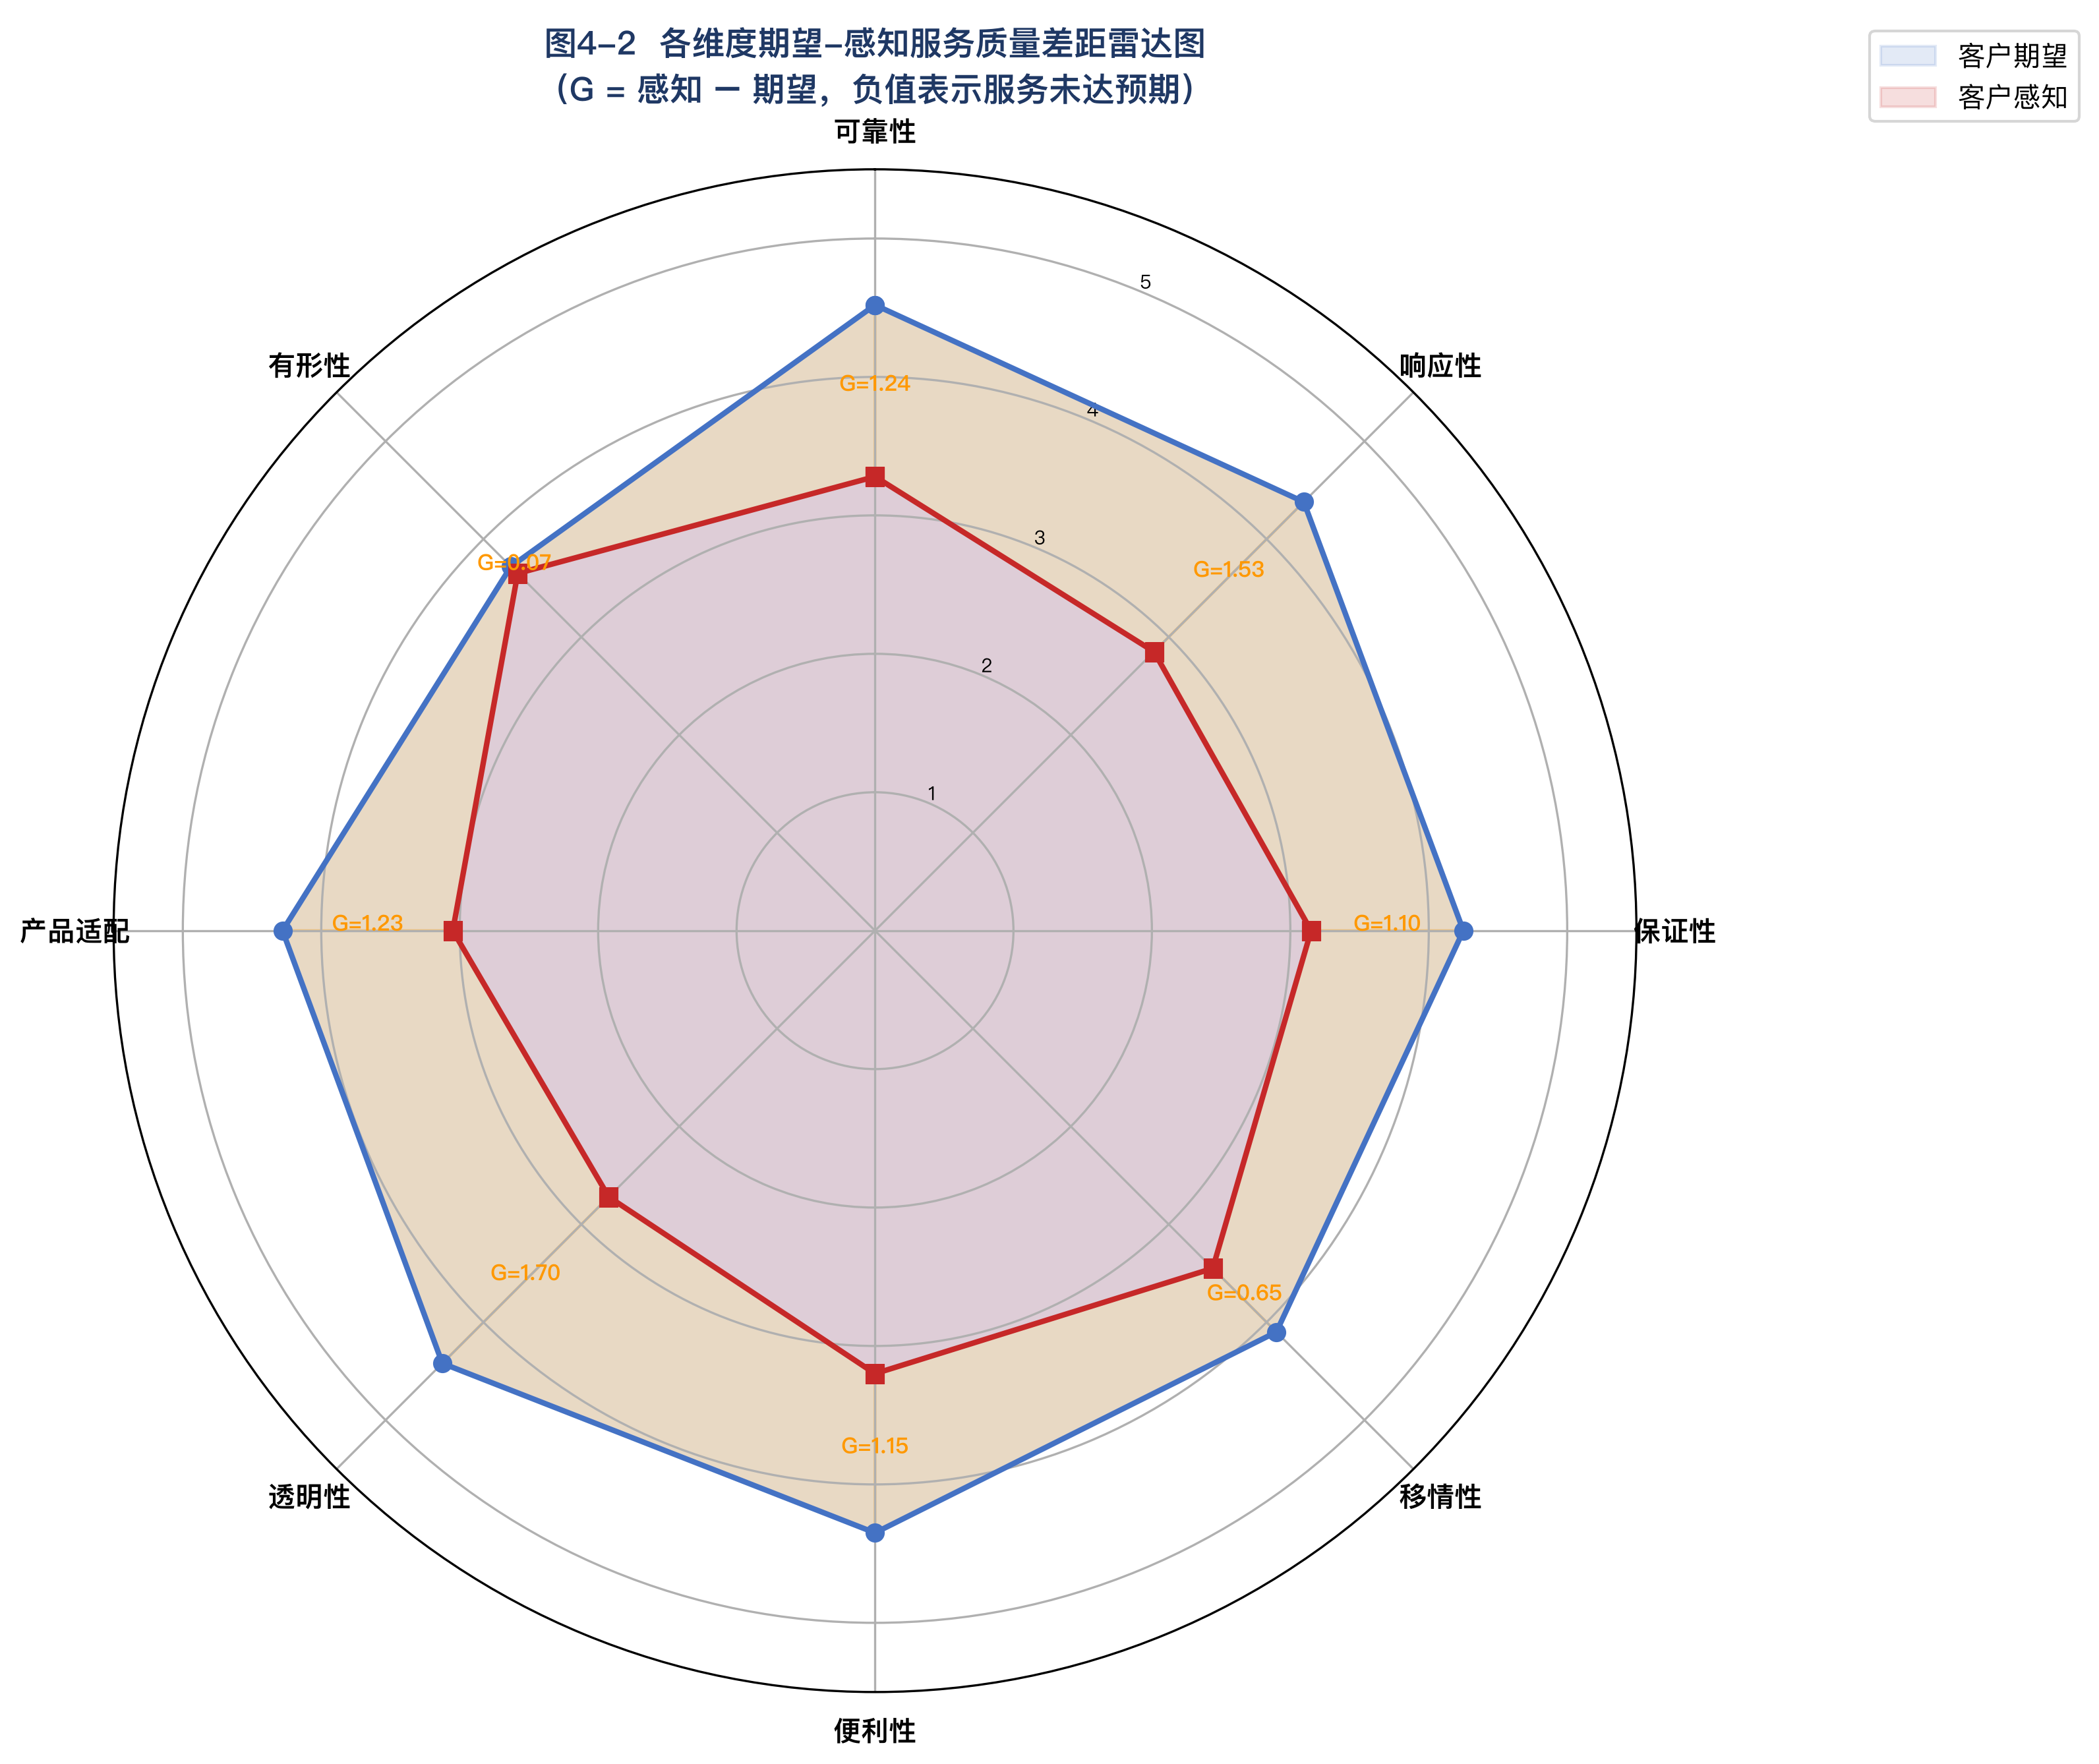
\includegraphics[width=0.85\textwidth]{figures/图4-3_期望感知差距雷达图.png}
  \caption{各维度期望-感知差距雷达图}
  \label{fig:4-3}
\end{figure}

对八组差距值进行配对样本t检验，结果显示各维度的感知均值均显著低于期望均值（$p < 0.01$），表明P公司小微贷款服务在所有评价维度上均存在不同程度的服务质量缺口。\par

从差距的绝对值来看，透明性维度的差距最大（$G = -1.70$），说明信息不对称是P公司小微贷款服务中最为突出的质量短板，客户对费用说明、审批进度和退件原因等核心信息的知情需求远未得到满足。响应性维度次之（$G = -1.53$），反映出客户对审批时效和响应速度的不满集中度较高。可靠性（$G = -1.24$）、产品适配（$G = -1.23$）、便利性（$G = -1.15$）和保证性（$G = -1.10$）的差距均超过-1.00，属于中等偏大的缺口区间，需要关注但紧迫性略低于透明性和响应性。移情性维度差距相对较小（$G = -0.65$），表明客户对P公司客户经理的个性化关怀认可度尚可。有形性维度的差距最小（$G = -0.07$），接近零差距，说明线下环境、合同规范和线上界面的服务质量接近于客户期望水平，不是当前阶段的核心矛盾。\par

\section{IPA/AHP权重与关键短板识别}

\subsection{IPA四象限分析}

IPA（Importance-Performance Analysis）分析方法将各评价指标的重要度（以期望均值表征）和满意度（以感知均值表征）绘制于二维坐标系中，以重要度均值（4.05）和满意度均值（3.42）为象限分界线，将全部指标划分为四个区域：优先改进区（高重要度-低满意度）、保持区（高重要-高满意）、供给过度区（低重要-高满意）和低优先区（低重要-低满意）。本文选取了15项具有代表性的关键服务质量指标进行IPA定位分析，各指标的坐标和象限归属如表4-2前半部分和图4-1所示。\par

\begin{table}[htbp]
  \centering
  \small
  \caption{关键服务质量指标IPA分析}
  \begin{tabularx}{\textwidth}{l c c l}
    \toprule
    \textbf{指标} & \textbf{重要度} & \textbf{满意度} & \textbf{象限} \\
    \midrule
    SQ01 审批时效承诺 & 4.52 & 2.95 & 优先改进 \\
    SQ18 材料一次告知 & 4.48 & 3.10 & 优先改进 \\
    SQ22 进度实时查询 & 4.35 & 3.25 & 优先改进 \\
    SQ23 退件原因明确 & 4.30 & 2.80 & 优先改进 \\
    SQ17 线上操作便捷 & 4.25 & 3.40 & 优先改进 \\
    SQ09 客户经理专业度 & 4.18 & 3.05 & 优先改进 \\
    SQ08 投诉处理效率 & 4.15 & 3.55 & 保持区 \\
    SQ25 贷款方案匹配度 & 4.10 & 3.15 & 优先改进（边界） \\
    SQ27 还款方式灵活 & 4.05 & 3.65 & 保持区 \\
    SQ15 贷后回访频率 & 3.98 & 3.75 & 保持区 \\
    SQ30 合同文件规范性 & 3.85 & 3.50 & 供给过度 \\
    SQ32 营业环境专业感 & 3.72 & 3.90 & 供给过度 \\
    SQ07 客服热线接通率 & 3.65 & 3.85 & 供给过度 \\
    客户活动频率 & 3.55 & 3.95 & 低优先 \\
    品牌宣传力度 & 3.45 & 3.70 & 低优先 \\
    \bottomrule
  \end{tabularx}
\end{table}

\begin{figure}[htbp]
  \centering
  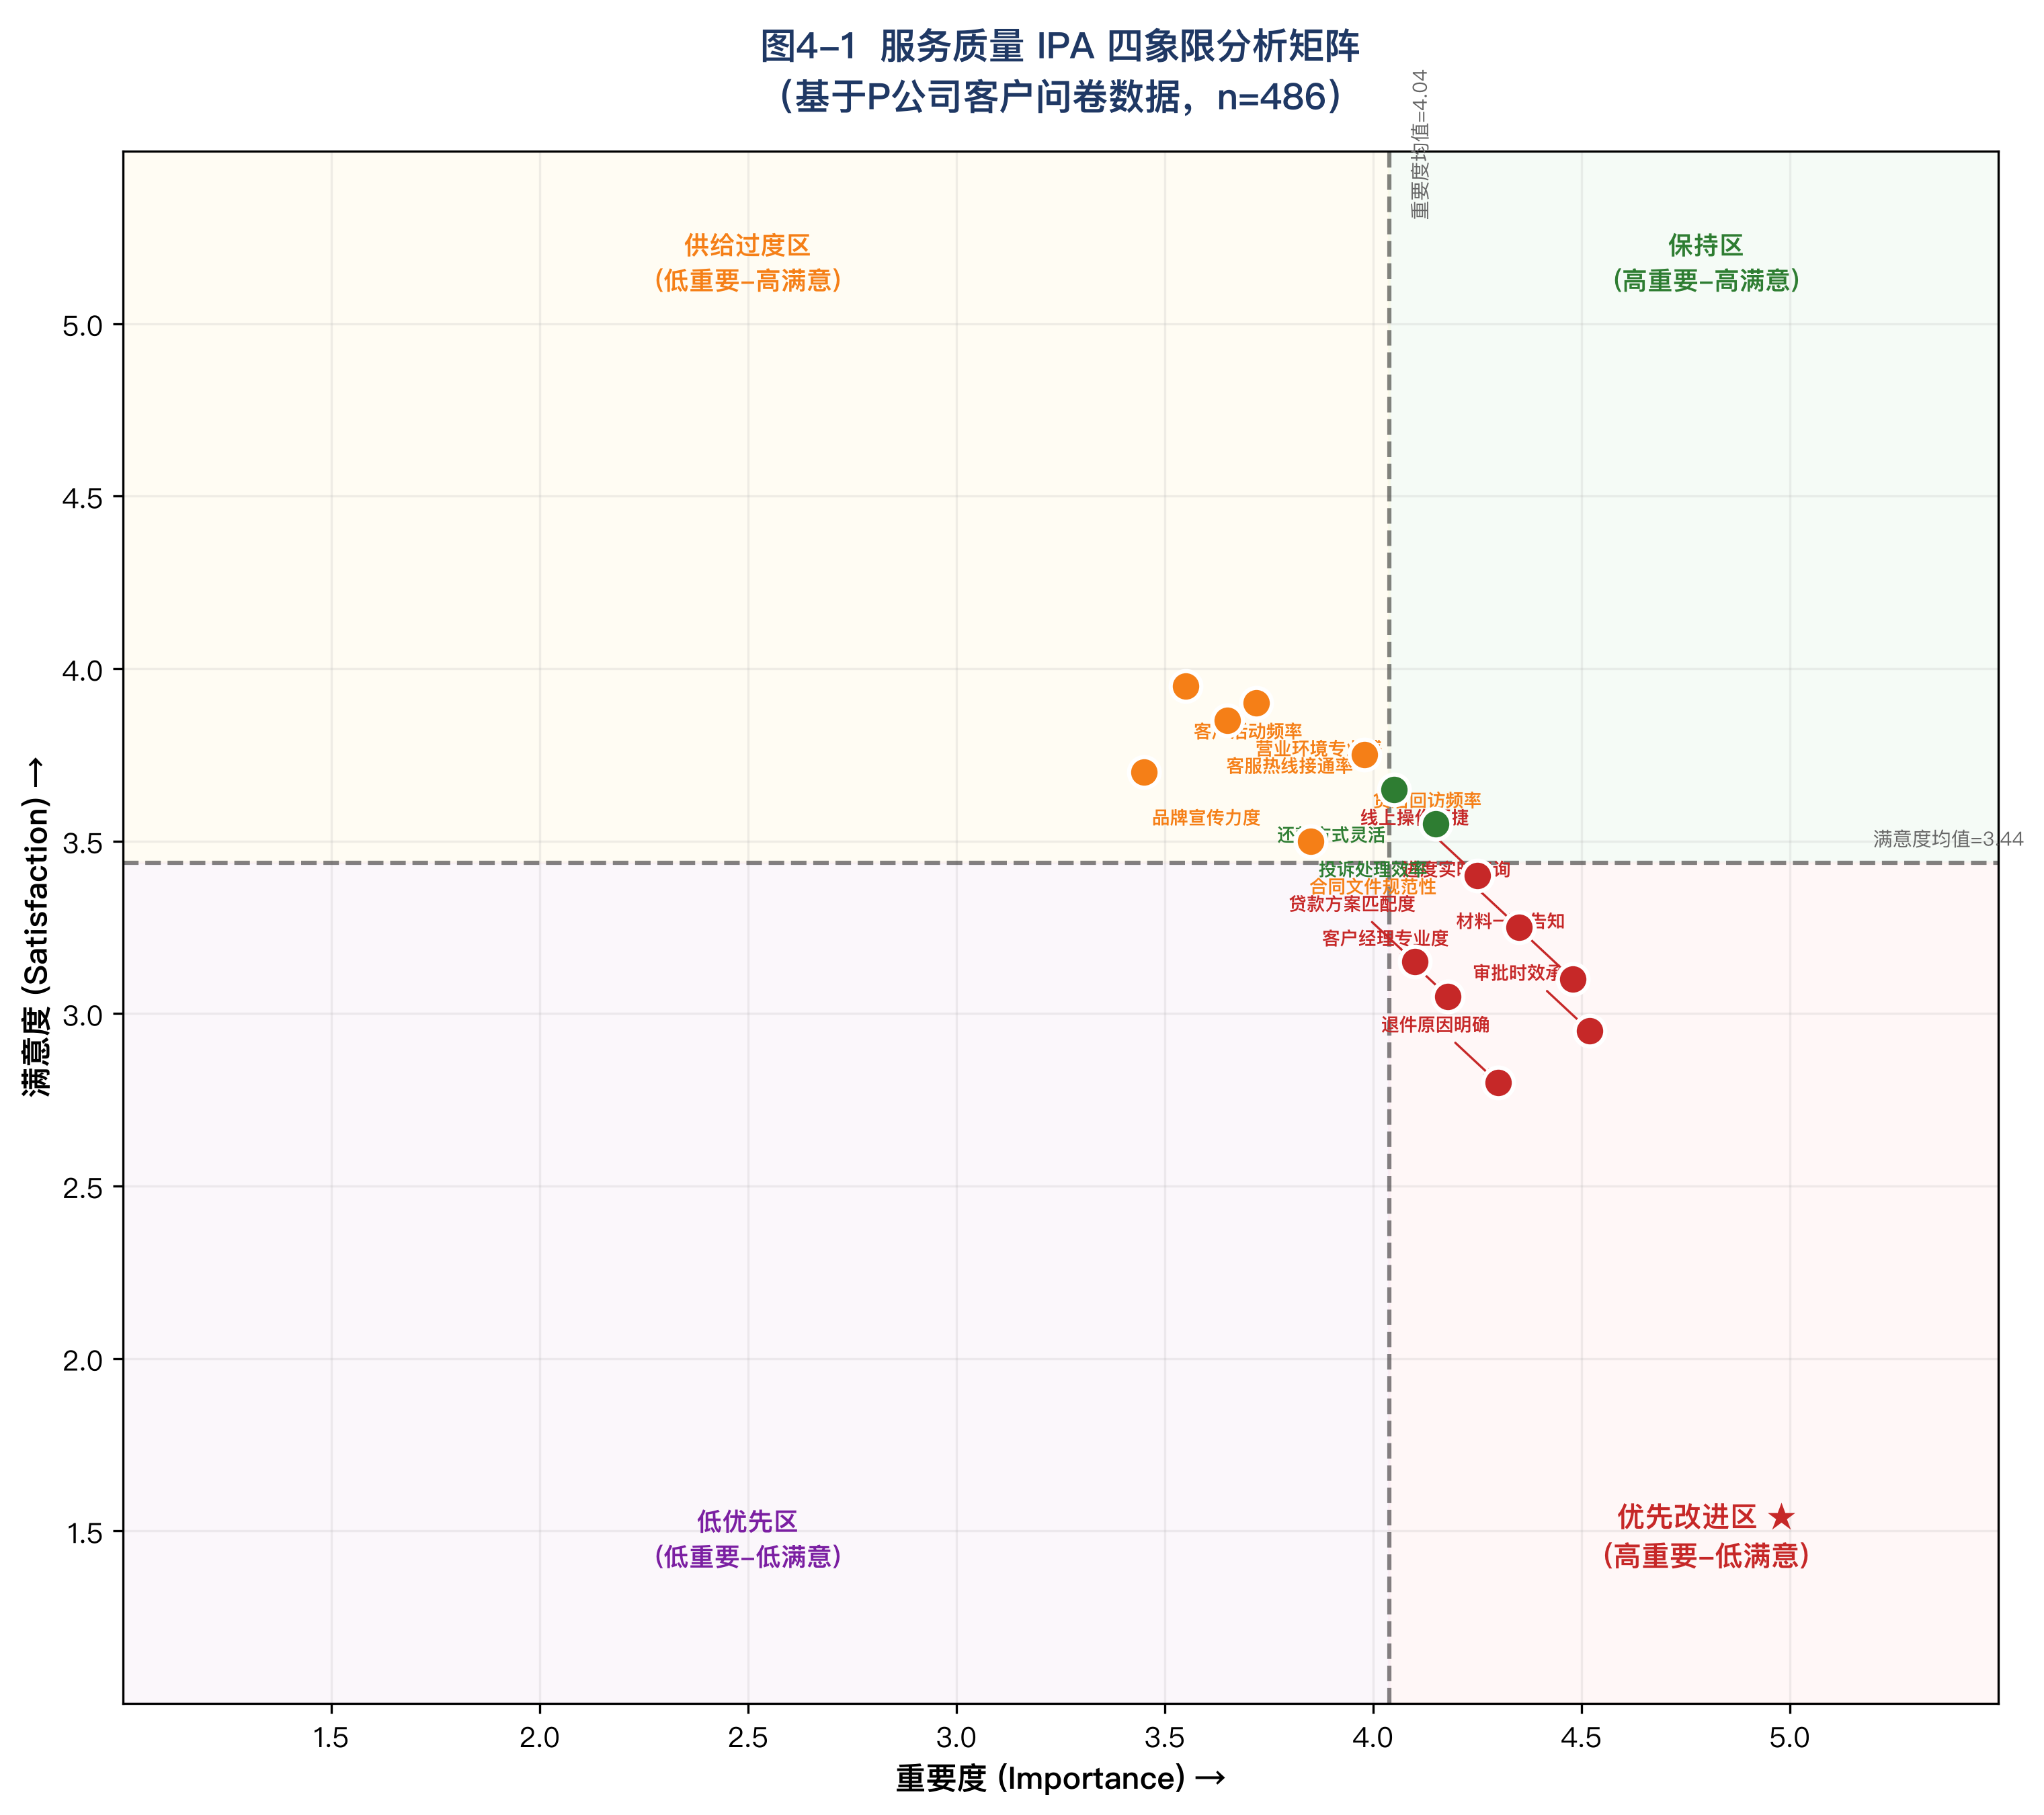
\includegraphics[width=0.85\textwidth]{figures/图4-1_IPA四象限分析矩阵.png}
  \caption{服务质量IPA四象限分析矩阵}
  \label{fig:4-1}
\end{figure}

由IPA分析结果可见，落入优先改进区的6项指标分别为：SQ01（审批时效承诺）、SQ18（材料一次告知）、SQ22（进度实时查询）、SQ23（退件原因明确）、SQ17（线上操作便捷）和SQ09（客户经理专业度）。这六项指标共同指向四个改进方向：信息透明化、流程简化、线上化体验优化和人员专业度提升。SQ25（贷款方案匹配度）处于优先改进区与保持区的边界，提示产品适配问题虽紧迫度略低于透明性和响应性，但仍构成不可忽视的质量短板。\par

供给过度区的三项指标（合同规范性SQ30、营业环境SQ32、热线接通率SQ07）和低优先区的两项指标（客户活动频率、品牌宣传力度）表明，P公司在这些方面的资源投入已超出客户的期望阈值，继续追加投入不会带来边际服务质量的显著提升，建议在后续的资源再配置中适当收缩以聚焦核心短板。\par

\subsection{AHP组合赋权}

为进一步量化各服务质量维度在整体评价中的相对重要性，本研究引入层次分析法（AHP）对八个服务质量维度进行专家赋权。AHP通过构建两两比较判断矩阵、计算特征向量和一致性比率（CR），将专家经验判断转化为定量权重，适用于多准则评价场景中的优先级排序。Nguyen等的研究验证了AHP与IPA组合方法在服务质量评价中的应用可行性\cite{ref30}，Moslem等的系统综述进一步证实了AHP在多准则决策中的稳健性\cite{ref31}。\par

Agrawal等（2022）提出的AHP-TOPSIS-DEMATEL组合方法为电子银行服务质量的多准则评价提供了系统化的方法论参照，证明AHP在多维服务质量评估中的适用性\cite{ref50}。\par

本研究邀请5位熟悉P公司小微贷款业务的客户经理和运营管理人员组成专家小组，基于八维服务质量框架进行维度间两两重要性比较。判断矩阵的专家意见经几何平均法聚合后计算出各维度的权重值，结果如表4-2所示。\par

\begin{table}[htbp]
  \centering
  \small
  \caption{AHP服务质量维度权重}
  \begin{tabular}{l c}
    \toprule
    \textbf{维度} & \textbf{权重} \\
    \midrule
    可靠性 & 0.185 \\
    响应性 & 0.172 \\
    透明性 & 0.158 \\
    便利性 & 0.142 \\
    产品适配 & 0.128 \\
    保证性 & 0.095 \\
    移情性 & 0.068 \\
    有形性 & 0.052 \\
    \bottomrule
  \end{tabular}
\end{table}

整体一致性比率CR值为0.038，低于0.10的阈值标准，表明专家判断矩阵通过了一致性检验，各维度权重值的可信度良好。\par

专家小组由5位P公司内部资深管理人员组成：2位运营高级经理、2位产品总监和1位风控总监，均具备五年以上小微信贷业务的一线管理经验。全部采用内部专家的考量在于：本研究聚焦P公司特定服务场景，小微信贷服务质量评价需要评审者深刻理解服务交付流程、目标客群特征和机构运营约束，内部专家的两两比较判断能够更准确地反映P公司实际运营中的维度重要性权衡。从AHP方法论标准审视，5位专家处于该方法论的最低可行规模边界\cite{ref31,ref39}；若以最大化权重估计的稳健性为目标，专家组应扩大至10至15人并纳入外部学术或行业评审者以补充多元视角。本研究判断矩阵一致性比率CR=0.038，低于0.10的接受阈值，表明五位内部专家在八维重要性排序上达到了良好的内部一致水平。\par

AHP赋权结果与IPA分析形成了有效印证：可靠性（0.185）、响应性（0.172）和透明性（0.158）分别位列权重前三，与IPA优先改进区的核心指标高度吻合；有形性（0.052）和移情性（0.068）的权重最低，与IPA分析中这两个维度的非紧迫定位一致。值得关注的是，透明性作为新增维度，其专家赋权名列第三，进一步验证了本文在SERVQUAL经典五维基础上增加透明性维度的必要性。\par

综合IPA四象限定位和AHP权重排序，本研究的测量结果表明，P公司小微贷款服务质量的优先改进方向应聚焦于：信息透明化（费用清晰、进度可查、退件明确）、流程响应加速（审批时效、进度通知）、线上操作体验优化和客户经理专业度提升。这四个方向对应了优先改进区六项关键指标的改进诉求，构成本文第5章根因分析和改进方案设计的核心输入。\par

\section{测量结果小结}

本章以改良SERVQUAL服务质量评价模型为工具，通过486份有效问卷数据完成了P公司小微贷款服务质量的系统测量。将测量结果中识别出的关键短板按优先级汇总，并与第5章的改进方案建立对应关系，如表4-3所示。\par

\begin{table}[htbp]
  \centering
  \small
  \caption{关键短板与改进方案对应关系}
  \begin{tabularx}{\textwidth}{c l c l X}
    \toprule
    \textbf{优先级} & \textbf{短板指标/维度} & \textbf{差距（$G$值）} & \textbf{IPA象限} & \textbf{对应改进方案} \\
    \midrule
    P1 & 透明性-退件原因明确（SQ23） & -1.70 & 优先改进 & 方案一：资料流程简化 \\
    P1 & 透明性-进度实时查询（SQ22） & -1.70（维度均值） & 优先改进 & 方案二：响应透明机制 \\
    P2 & 响应性-整体维度 & -1.53 & 优先改进 & 方案二：响应透明机制 \\
    P2 & 可靠性-审批时效承诺（SQ01） & -1.24（维度均值） & 优先改进 & 方案一：资料流程简化 \\
    P3 & 产品适配-维度 & -1.23 & 优先改进（边界） & 方案三：客户分层适配 \\
    P4 & 便利性-线上操作（SQ17） & -1.15 & 优先改进 & 方案一 + 方案二 \\
    P5 & 保证性-客户经理专业度（SQ09） & -1.10 & 优先改进 & 方案四：客户经理能力 \\
    \bottomrule
  \end{tabularx}
\end{table}

上述短板分类呈现出三个结构性特征：其一，信息透明和响应速度构成了P公司小微贷款服务的最核心短板群（P1—P2），两项短板相互交织——退件原因不明确导致客户反复补正材料，进而拉长审批周期、加剧响应性维度差距；其二，产品适配和线上操作体验构成次优先级短板群（P3—P4），反映了标准化服务模式与小微客户异质性需求之间的结构性张力；其三，客户经理专业度（SQ09）的IPA坐标（重要度4.18，满意度3.05）明确落入优先改进区，表明客户对客户经理专业能力的期望与实际感知之间存在显著落差，该结论与AHP专家赋权中保证性维度的权重共同构成本文第5章方案四（客户经理专业度提升）的定量依据。从DMAIC方法论的视角审视，上述短板识别结果已完成了测量阶段的核心使命——将P公司服务质量的模糊痛感转化为可量化、可排序、可追溯的管理指标。每一优先级的短板均有明确的数值锚点（G值）、空间定位（IPA象限）和权重支撑（AHP维度权重），使得第5章的根因分析和改进方案设计不再是经验驱动的试错，而是数据驱动的工程化决策。\par

本章完成了DMAIC方法论"测量"阶段的核心任务——从模型选择到问卷实施，再到信效度检验和IPA/AHP短板识别，产出了一套完整的小微贷款服务质量量化测量结果。这些结果为第5章基于DMAIC方法的根因分析和改进方案设计提供了明确的定量导向和优先序依据。\par

\section{研究局限}

本章的研究在方法论层面存在以下局限，需要在解读数据结果时加以审慎考量。\par

\subsubsection{因子分析方法}

本研究选择EFA而未执行CFA，其方法论依据包括：第一，将SERVQUAL适配于小微信贷场景属探索性研究，尚无成熟因子结构可供预设，EFA的数据驱动特性与这一研究阶段相符；第二，八因子32题项的CFA结构需400至500份以上样本方可稳定估计\cite{ref21}，n=486正处于该区间下限且已全部用于EFA；第三，先探索后验证的方法论路径（先EFA后CFA）在量表开发研究中为常规做法。建议未来研究以独立样本（$n \geq 500$）执行CFA，报告CFI、TLI、RMSEA等模型拟合指数，并辅以组合信度（CR）、平均方差提取量（AVE）和区分效度检验，以全面验证八维结构的测量效度。\par

\subsubsection{共同方法偏差}

期望值与感知值由同一问卷在同一时间点采集，存在共同方法偏差（Common Method Bias, CMB）风险——自变量与因变量均来自同一测量来源和测量语境，可能人为放大变量间的相关程度。本研究通过Harman单因子检验对CMB进行了初步评估（未旋转的单因子最大方差解释率低于50\%的临界值），但尚不能完全排除CMB对结论的潜在影响。未来研究可采用多源多时点设计（如将期望值与感知值分阶段采集）减少CMB，或引入客户行为数据等客观指标作为交叉验证。\par

\subsubsection{研究者角色}

研究者在P公司担任服务质量改进项目负责人，对业务背景和流程痛点的深入理解有助于提升诊断的精准度，但同时也可能引入研究者偏差（Researcher Bias）——在指标选取、根因判断和方案优先级排序中不自觉地倾向于与自身经验一致的假设。为减少此影响，本研究采取了以下措施：问卷采用完全匿名形式发放，客户被告知调查数据仅用于学术研究目的且与P公司业务决策无关；数据分析由独立第三方统计学顾问协助完成SPSS处理和结果解读，研究者本人未直接操作原始数据清洗和分析脚本。尽管如此，研究者在问卷设计和改进方案设计中的主体角色意味着绝对客观性难以完全保证，读者应结合此背景解读研究结论。\par

\subsubsection{样本局限与非回应偏差}

本研究面向P公司近12个月活跃客户发放问卷800份，回收有效问卷486份，有效回收率60.8\%，存在39.2\%的非回应率。未回应客户的服务质量评价可能系统性地不同于回应客户：对P公司服务体验极度不满并已终止合作的客户可能拒绝参与调查，而对服务质量漠不关心的客户可能因缺乏参与动机而未填写问卷，两者对总体服务质量估计值的净影响方向难以确定。此外，486份有效样本的地域分布和行业构成受P公司既有业务覆盖范围决定，其代表性受限于P公司的客户结构特征，在将结论推广至更广泛的小微贷款客户总体时需保持审慎。非回应偏差的存在意味着本文报告的差距分值可能在一定程度上偏离P公司全体活跃客户的实际服务质量感知水平，建议在解读各维度差距值的绝对值时考虑这一测量不确定因素。\par

\subsubsection{AHP专家小组规模}

本研究AHP赋权的专家小组由5位成员组成，全部为P公司内部管理人员（运营高级经理2位、产品总监2位、风控总监1位）。5位专家处于AHP方法论的最低可行规模\cite{ref31,ref39}，低于10至15人的理想区间。首先，小规模专家组对个别专家的极端判断更为敏感，任何一位评审者的评分偏移都可能对最终权重产生不成比例的影响。其次，全部专家均来自P公司内部，虽然保障了评审者对小微信贷业务的深度理解，但也引入了潜在的组织内聚偏差——五位成员长期在同一组织中协作，可能在管理优先级、客户感知假设和资源分配逻辑上存在系统性趋同，导致判断矩阵的一致性（CR=0.038）虽低于0.10阈值，但可能部分反映的是共享组织视角而非维度间客观重要性的独立共识。第三，专家判断嵌入了P公司特定运营阶段的优先序，在推广至其他普惠金融机构或P公司的不同发展阶段时需重新校准。建议未来研究将专家组扩大至10至15人，纳入外部行业专家、监管机构代表和学术评审者，并采用Delphi多轮反馈机制以减少组织内聚偏差，增强权重的代表性和外部效度。\par

\subsubsection{单一案例局限}

本研究以P公司为单一案例对象，其服务质量评价模型的维度权重、IPA象限指标分布和DMAIC改进方案的参数设计均以P公司的组织特征（持牌普惠金融公司、线上线下双渠道运营、45人客户经理团队规模）为经验基础。不同普惠金融机构在牌照类型、线上化程度、目标客群特征和风险管理模式上的差异，可能导致服务质量维度结构的权重重新排序和改进方案优先级的调整。因此，本文的研究发现——尤其是八维SERVQUAL模型的具体权重值和五个改进方案的参数设定——不宜直接套用至其他机构，但本研究所构建的"改良SERVQUAL测量$-$IPA/AHP组合赋权$-$DMAIC闭环改进"方法论框架具有较强的可迁移性，可作为同类机构开展服务质量改进的参考模板。\par

\section{引用落点表}

\begin{table}[htbp]
  \centering
  \small
  \caption{第4章引用落点表}
  \begin{tabularx}{\textwidth}{l l X l l}
    \toprule
    \textbf{引用编号} & \textbf{使用位置} & \textbf{支撑观点} & \textbf{证据类型} & \textbf{状态} \\
    \midrule
    [21] & 4.1 模型选择；4.2 指标体系；4.4 效度分析 & SERVQUAL期望-感知差距模型的理论基础 & PDF & 已入库 \\
    [6] & 4.1 模型选择；4.4 效度分析；4.5 IPA分析 & SERVQUAL-IPA在金融机构服务质量评价中的应用参照 & PDF & 已入库 \\
    [26] & 4.1 模型选择 & 服务质量-满意度-忠诚度关系链支撑 & PDF & 已入库 \\
    [29] & 4.2 指标体系 & e-SERVQUAL线上服务质量维度扩展参照 & 元数据 & 已入库 \\
    [24] & 4.2 指标体系 & 数字银行满意度维度参照 & Web\_MD & 已入库 \\
    [25] & 4.2 指标体系 & 数字银行体验与风险维度的实证参照 & Web\_MD & 已入库 \\
    [12] & 4.2 指标体系；4.3 问卷设计 & 国内银行网点服务质量指标设计和问卷构造方法 & PDF（学位论文） & 已入库 \\
    [11] & 4.2 指标体系；4.3 问卷设计 & 银行对公业务满意度和AHP问卷设计经验 & 元数据（学位论文） & 已入库 \\
    [18] & 4.3 问卷设计 & 银行小微客户关系管理中客户分层抽样策略 & PDF（学位论文） & 已入库 \\
    [内部数据] & 4.2 指标体系；4.3 问卷设计；4.4 效度分析 & P公司内部数据、客户访谈反馈和研究授权 & 内部数据 & 已脱敏 \\
    [30] & 4.5 IPA/AHP分析 & IPA/AHP组合方法在服务质量评价中的应用验证 & 元数据 & 已入库 \\
    [31] & 4.5 IPA/AHP分析 & AHP多准则评价的系统综述和稳健性支撑 & 元数据 & 已入库 \\
    [39] & 4.5.2 AHP赋权；4.7 研究局限 & AHP层次分析法方法论标准与权重稳健性支撑 & 期刊 & 已入库 \\
    \bottomrule
  \end{tabularx}
\end{table}
